\chapter{Data Fitting}\label{ch:data-fitting}

In many numerical methods, we evaluate a function $f(x)$ at a set of sampling points $x_i,\, i=0, \cdots, N$.  We have been using the set of function values $F_i=f(x_i)$ as a discrete expression of the function.    Now, we consider the opposite operation.
Suppose that we are given a data set $(x_i, F_i),\, i=0,\cdots, N$.  Can we find the original function $f(x)$?  Strictly speaking, that is not possible. Since the data set provides only a limited information, there is no way to define a unique function.  Many different functions can generate the same data set.  Nevertheless, we want to find a function with the help of additional conditions. This is the data fitting problem.

The fitting methods depend on what you want to learn from the data.   There are two major different classes of problems.  
In one class,
we want to know the function value between the data points.  What is the value of $f(x)$ at $x$ between $x_i$ and $x_{i+1}$?   This is the interpolation problem.  In some cases, we also want to know the derivative of the function.  Of course we have no way to know it exactly. Therefore, we have to assume various properties of the function.  The minimum requirement is that the function must be continuous. In addition, the continuity of $f'(x)$, and $f''(x)$ can be optionally required.  In most cases, our focus is on the small region and we don't need to find $f(x)$ for the wide range of $x$. Piece-wise polynomials are good enough to fill the gap between data points.  Such methods are called \textit{spline}.   Usually, this kind of problems assume that the data points are exact and thus all data points must be exactly on the fitted curve.  On the other hand, the function $f(x)$ not necessary corresponds to a theoretical prediction based on physics.  We just want to express the discrete data sets with a continuous function so that we can find the function values between the data points.

The second kind of problem is quite different.  We know the type of function $f(x)$ predicted by a theory or by a conjecture, say, a Gaussian function.  We want to compare the prediction with the data set obtained by an experiment.  However, the function often contains parameters whose values are unknown.  For the Gaussian function, the mean and variance are the parameters. If the theory is correct, we should be able to determine the parameter values by fitting the parameter values to the experimental data.  Unlike the previous problems, the data set is usually noisy and erroneous.  It is not necessary to fit the function exactly to the data.  Furthermore, the number of parameters are much smaller than the size of the data set.  It is not possible to satisfy all conditions by adjusting a few parameters. Therefore, the ``fitness'' is not uniquely defined.  In statistics, this kind of analysis is called \textit{regression}.  In general this is an optimization problem. 

In this chapter we discuss the two classes of the problems, spline and least square fitting.  More advanced optimization methods will be used in Chapter 18.

\section{Spline}

Consider a data set ($x_i$, $F_i$), $i=0, \cdots, N$.  We expect that these data are sampled from an continuous function $f(x)$. However, we have no knowledge of the function. We want to find the function so that we can see the function values between data points. 
However, there is no way to determine the function uniquely since we have only a finite number of the data. There are infinitely many functions which match to the data.  Therefore,  we need further assumptions.  We consider two different approaches.  In one approach, we assume that $f(x)$ is a polynomial of order $N$.  This single function covers the whole region $x \in [x_0, x_\textsc{N}]$. We will discuss this approach later.
The other approach uses a different function for each segment.  For the segment  $x \in [x_i, x_{i+1}]$, we introduce a function
$f_i(x)$. Usually, information given in the data set is not enough to determine the function and some additional conditions are needed for this approach.

\subsection{Linear Spline}

We begin with the simplest spline.  This method is not very useful in practice but leads us to a better method. 
For simplicity, we introduce a new variable 
\begin{equation}
t = \frac{x-x_i}{h_i}, \qquad t \in [0,1]
\end{equation}
where the gap distance between $x_i$ and $x_{i+1}$ is denoted as $h_i = x_{i+1}-x_i$.  When $x$ varies from $x_i$ to $x_{i+1}$, $t$ changes from $0$ to $1$. 

Between two adjacent points $x_i$ and $x_{i+1}$,  we assume that the function takes a linear form
\begin{equation}\label{eq:spilne_linear1}
f_i(t) = a_i t + b_i\,.
\end{equation}
The function must agree with the data points and thus
\begin{equation}\label{eq:spline_rule1}
f_i(0) = F_i, \qquad f_i(1)=F_{i+1}
\end{equation}
which is the mandatory condition.  These two conditions are sufficient to determine the parameters $a_i$ and $b_i$. No other conditions are needed.  We immediately find $a_i = F_{i+1}-F_i$ and $b_i = F_i$ and thus the function is.
\begin{equation}\label{eq:spline_linear2}
f_i(t) = (1-t) F_i + t F_{i+1}
\end{equation}
which interpolates the function values between the two data points.

The present scheme simply connects data points by straight lines as we do when we plot a data. 
A major draw back of this method is that the function is not smooth at every data point. (See Example ) 
The required condition (\ref{eq:spline_rule1}) guarantees that the function is continuous but its derivative is not necessarily continuous.  WE could impose additional condition such that the derivative is continuous at the data points.  However, the parameters $a_i$ and $b_i$ in the linear interpolation (\ref{eq:spilne_linear1}) are already uniquely determined by the condition (\ref{eq:spline_rule1}.  There is no room to impose additional conditions.  Therefore, higher order polynomials must be used if we need a smooth function,

\begin{example}\label{ex:spline_linear}

\begin{table}
\centering
\caption{Data for polynomial fitting}\label{tbl:spline_data}
\begin{tabular}{c | c c c c c c}
\hline
x & 0 & 1 & 2 & 3 & 4 & 5\\
\hline
F & 0.0000& 0.6889& 0.6095& 0.0774& -0.3401& -0.3528\\
\hline\hline
x  & 6 & 7 & 8 & 9 & 10 & \\
\hline
F  & -0.0842& 0.1620& 0.1997& 0.0681& -0.0736 &\\
\hline
\end{tabular}
\end{table}

A data set is given in Table \ref{tbl:spline_data}.   We will interpolate between these data points by linear functions. Program \ref{prog:spline_linear} uses 
Eq. (\ref{eq:spline_linear2}) to fill the gap between the data points.  The result is shown in Fig. \ref{fig:spline_linear}.   Although all data points are exactly connected, the curve is not smooth at the data points.  The data (Table  \ref{tbl:spline_data}) is actually sampled from $\sin(x) \me^{-x/5}$, which is the dashed line in Fig. \ref{fig:spline_linear}.  The large difference between the linear spline and the original function is seen hear the maxima and minima of the function.  A high order method is needed to improve it.
\end{example} 

\subsection{Cubic Spline}

In order to make it sure that the function is smooth, we require that the first and second order derivatives are continuous.
A function  $f_i(t)$ interpolates between  the two points $x_i$ and $x_{i+1}$. In addition to the mandatory conditions (\ref{eq:spline_rule1}), we impose
\begin{eqnarray}
f'_{i-1}(1) = f'_i(0), &\qquad & f'_i(1)=f'_{i+1}(0) \label{eq:spline_rule2}\\
f''_{i-1}(1) = f''_i(0), &\qquad & f''_i(1)=f''_{i+1}(0)  \label{eq:spline_rule3}
\end{eqnarray}
where the single and double prime indicate the first and second order derivatives, respectively.
These four additional conditions allows two more parameters in $f_i(t)$. (Note that these conditions are shared by the neighboring segments and thus only two additional degrees of freedom are allowed.)  Therefore, $f_i(t)$ must be a cubic function of $t$.

Detailed derivation is given in Appendix.  Here we show the final result.  The following function satisfied three conditions
(\ref{eq:spline_rule1}), (\ref{eq:spline_rule2}) and (\ref{eq:spline_rule3}).
\begin{equation}\label{eq:spline_cubic}
f_i(t) = \frac{h_i^2}{6} t (t+1)(t-1) Q_i -  \frac{h_i^2}{6} t (t-1)(t-2) Q_{i+1} + (1-t) F_i + t F_{i+1}, \quad i=0, \cdots, N-1
\end{equation}
where $Q_0=Q_\textsc{N}=0$ and remaining $Q_i$ is the solution of linear equation
\begin{equation}\label{eq:spline_cubic_params}
\begin{bmatrix}
d_1    & h_1 & 0      & \cdots         &  0 \\
h_1    & d_2 & h_2    &                &  0 \\
0      & h_2 & d_3    & \ddots         &  \vdots \\
\vdots &     & \ddots & \ddots         &  h_\textsc{N-2} \\
0      &  0  & \cdots & h_\textsc{N-2} &  d_\text{N-1} 
\end{bmatrix}
\begin{bmatrix}
Q_1 \\ Q_2 \\ \vdots\\ Q_\textsc{N-2} \\ Q_\textsc{N-1}
\end{bmatrix}
=
  \begin{bmatrix}
G_1 \\ G_2 \\ \vdots\\ G_\textsc{N-2} \\ G_\textsc{N-1}
\end{bmatrix}    
\end{equation}
where $d_i=\displaystyle\frac{1}{2} (h_i+h_{i-1})$ and $G_i = 3 \left ( \displaystyle\frac{F_{i+1}-F_i}{h_i} - \displaystyle\frac{F_i-F_{i-1}}{h_{i-1}} \right )$. The matrix in Eq (\ref{eq:spline_cubic_params}) is tridiagonal, which makes it relatively easy to solve the equation for a large data set.  This is one reason cubic spline is popular.

\begin{example}
We fits the data in Example \ref{ex:spline_linear} using cubic spline.  Program \ref{prog:spline_cubic}  solves the linear equation (\ref{eq:spline_cubic_params}) and constructs the cubic functions (\ref{eq:spline_cubic}).  The result is shown in Fig. \ref{fig:spline_cubic}.  The curve is now smooth and looks more natural than the linear spline.

\begin{figure}
	\centering
	\begin{subfigure}{0.45\textwidth}
		\centering
		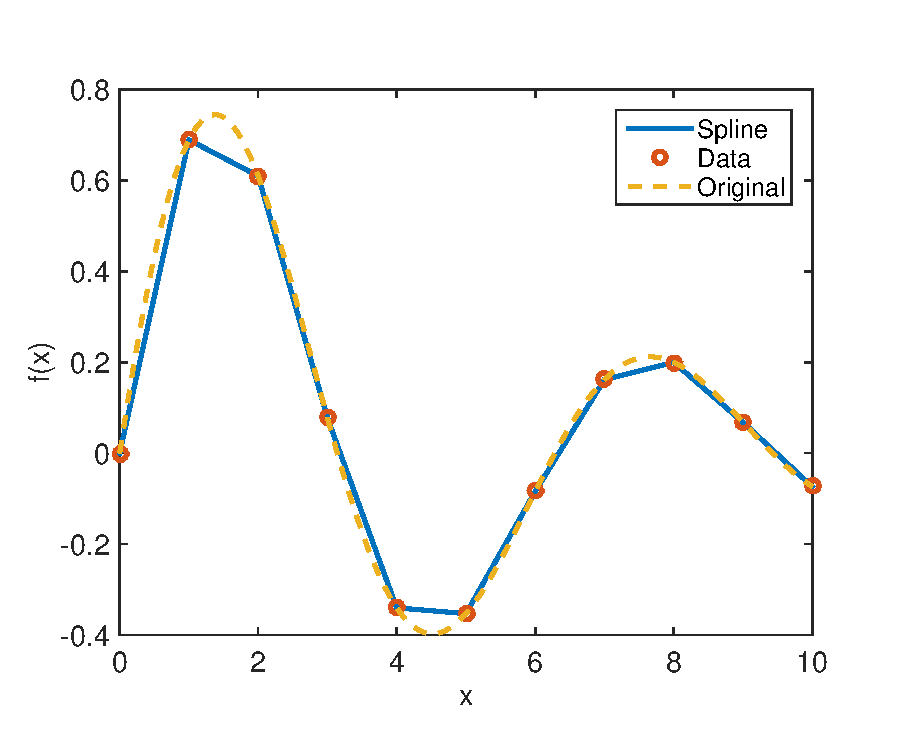
\includegraphics[width=2.5in]{12.fitting/spline_linear.pdf}
		\caption{Linear spline:  The linear interpolation is continuous but it is not smooth at every data point.  In particular, it looks bad near the extrema.}
		\label{fig:spline_linear}
	\end{subfigure}
	\begin{subfigure}{0.45\textwidth}
		\centering
		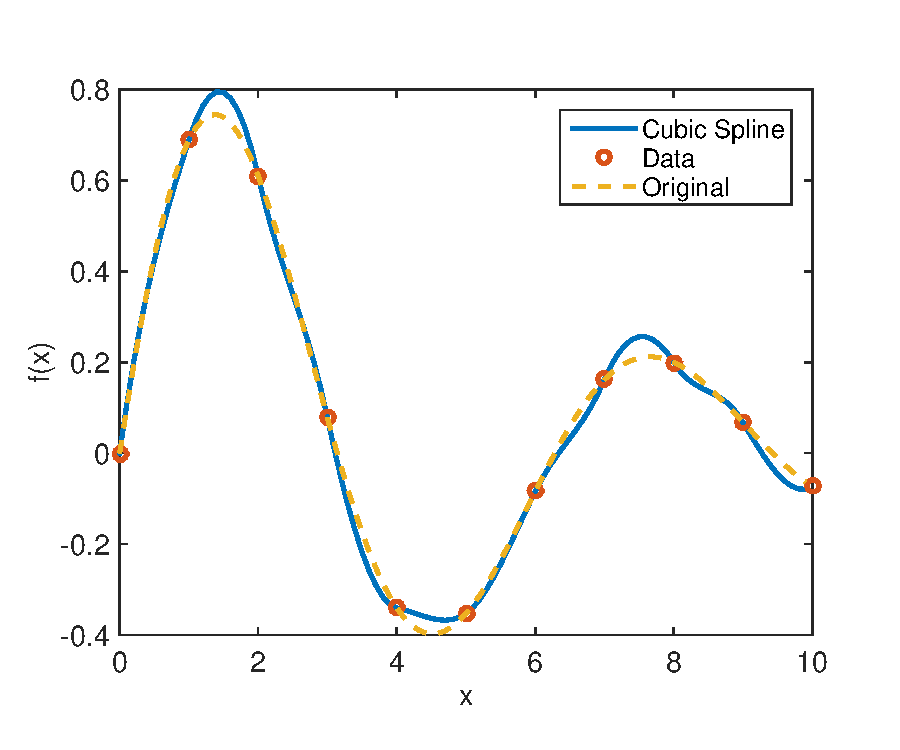
\includegraphics[width=2.5in]{12.fitting/spline_cubic.pdf}
		\caption{Cubic spline: The curve is now smooth.}
		\label{fig:spline_cubic}
	\end{subfigure}
\caption{Linear and cubic spline of the data given in Exampel \ref{ex:spline_linear}. The dashed curve is the original function from which the data set was generated.}
\end{figure}

\end{example}

\noindent
\subsection{Vandermonde matrix}

Since we are given $N+1$ data, we can, in principle, determine $N+1$ unknown parameters. Thus we can interpolate the data with a polynomial of degree $N$,
\begin{equation}
f(x) = a_0 + a_1 x + a_2 x^2 + \cdots a_\textsc{N} x^{N}.
\end{equation}
The fitting rule is simply $f(x_i)=F_i,, \quad \forall i$.
Substituting the data points to this equation, we have a set of equations that the coefficients $a_i$ must satisfy,
\begin{equation}
F_i = a_0 + a_1 x_i + a_2 x_i^2 + \cdots +a_\textsc{N} x^{N}, \quad i=0, \cdots, N
\end{equation}
which can be written in a matrix form $X \mathbf{a} = \mathbf{f}$ where
\begin{equation} \label{eq:vandermonde_matrix}
X = \begin{bmatrix}  
1 & x_0 & x_0^2 & \cdots & x_0^{N} \\
1 & x_1 & x_1^2 & \cdots & x_1^{N} \\
  &     &       & \vdots &           \\
1 & x_\textsc{N-1} & x_\textsc{N-1}^2 & \cdots & x_\textsc{N}^\textsc{N}
\end{bmatrix}, \quad
\mathbf{a} = \begin{bmatrix} a_0 \\ a_1 \\ \vdots \\ a_\textsc{N} \end{bmatrix}, \quad
\mathbf{f} = \begin{bmatrix} F_0 \\ f_1 \\ \vdots \\ F_\textsc{N} \end{bmatrix}.
\end{equation}
Then the solution is $\mathbf{a} = X^{-1} \mathbf{f}$.  The matrix $X$ is called the Vandermonde matrix.

In general the Vandermonde matrix is not a nice matrix to solve due to round-off errors which grows as $N$ increases.  In addition, unlike  the tridiagonal matrix for the cubic spline method, the Vandermonde matrix is not a sparse matrix and it takes longer time to solve Eq. (\ref{eq:vandermonde_matrix}).

\bigskip
\begin{example}[Vandermode matrix]\label{ex:Vandermonde}

We fit the data in Table \ref{tbl:spline_data} again.  This time we fit the data to a polynomials of degree 10 using the Vandermonde method.  Program \ref{prog:vandermonde} implements the above method and the result is plotted in Fig. \ref{fig:vandermonde}.  The fitted curve looks more natural than the cubic spline (Fig. \ref{fig:spline_cubic}).  It is essentially identical to the original function from which the data set was genrated.

\medskip
The following code executes the above method.  The result is plotted in Fig. \ref{fig:vandermonde}.  The curve passes through the given data points precisely as it should.  However, the interpolation is reasonable only between $x=3$ and $x=7$. Suspicious dips can be seen between $x=0$ and $x=1$ and also between $x=9$ and $x=10$.  Off course, we cannot tell that those are false.  Simply we don't have sufficient data to interpolate near the boundaries. However, those dips violate our underlying assumption.  Therefore, we conclude that the interpolation is good only in the central region.
In this example, the Vandermonde matrix is able to fit the data very well. 

\begin{figure}
\centering
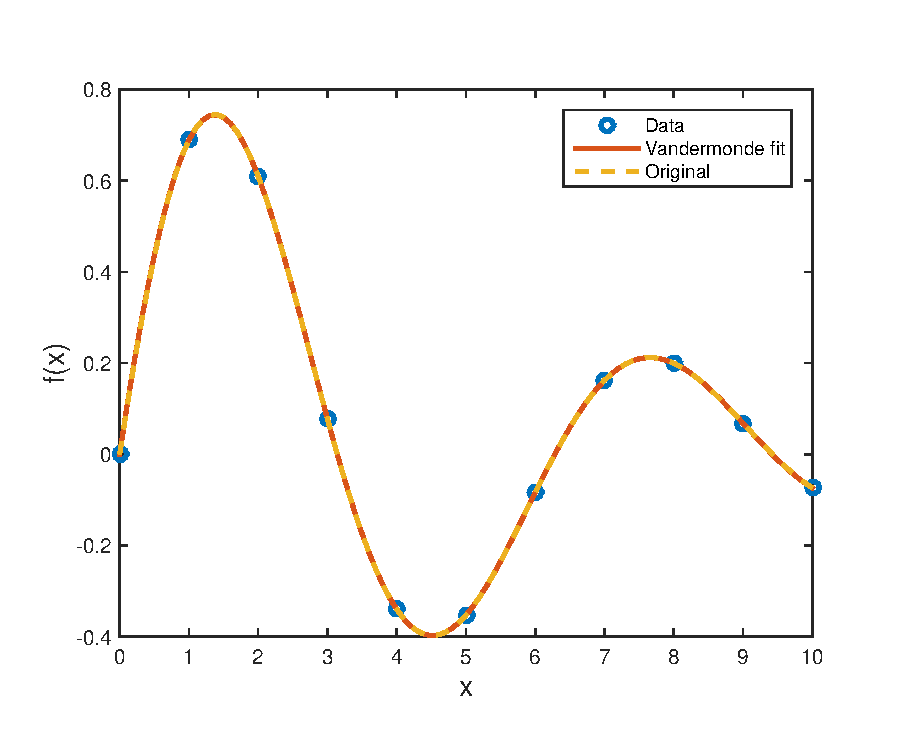
\includegraphics[width=2.5in]{12.fitting/vandermonde.pdf}
\caption{Polynomial Fitting of random data given in Table \ref{tbl:spline_data}.  The open circles show the original data and the line plots the interpolation by the polynomial obtained by the Vandermonde matrix.}\label{fig:vandermonde}
\end{figure}
\end{example}


\noindent
\subsection{Lagrange Polynomial}

There is another way to determine the coefficients of the polynomial.  Expanding the function near the sampling point,
\begin{equation}
F_i  = f(x_i) = f(x) + (x-x_i) f'(x) + \frac{1}{2} (x-x_i)^2 f''(x) + \cdots, \qquad i=0, \cdots, N
\end{equation}
Since there is $N+1$ equations, we can solve them for $f(x)$, $f'(x)$, ..., $f^{(N)}(x)$.  For example if $N=1$,
we have two equations upto the first order derivatives
\begin{subequations}
\begin{eqnarray}
F_0 &=& f(x) + (x-x_0) f'(x) \\
F_1 &=& f(x) + (x-x_1) f'(x) 
\end{eqnarray}
\end{subequations}
Solving these equations for $f(x)$, we just get Eq. (\ref{eq:spline_linear2}). For $N=2$, we include the second order derivatives and the equations to solve is given by
\begin{subequations}
\begin{eqnarray}
F_0 &=& f(x) + (x-x_1) f'(x) + \frac{1}{2} (x-x_1)^2 f''(x) \\
F_1 &=& f(x) + (x-x_2) f'(x) + \frac{1}{2} (x-x_2)^2 f''(x) \\
F_2 &=& f(x) + (x-x_3) f'(x) + \frac{1}{2} (x-x_3)^2 f''(x)
\end{eqnarray}
\end{subequations}
and the solution is
\begin{equation}
f(x) = \frac{(x-x_2)(x-x_3)}{(x_1-x_2)(x_1-x_3)} F_0
+\frac{(x-x_1)(x-x_3)}{(x_2-x_1)(x_2-x_3)} F_1
+\frac{(x-x_1)(x-x_2)}{(x_3-x_1)(x_3-x_2)} F_2
\end{equation}
which is equivalent to the quadratic fitting. 

The solution for general $N$ is known as Lagrange polynomials
\begin{equation}
f(x) = \sum_{n=0}^{N} \ell_n(x) F_n
\end{equation}
where Lagrange basis polynomials are defined by
\begin{eqnarray}
\ell_n(x) &=& \prod_{m=0, m\ne n}^{N} \frac{x-x_m}{x_n-x_m} \\
&=& \frac{(x-x_1)}{(x_n-x_1)}\cdot \frac{(x-x_2)}{(x_n-x_2)} \cdots \frac{(x-x_{n-1})}{(x_n-x_{n-1})} \cdot 
\frac{(x-x_{n+1})}{(x_n-x_{n+1})} \cdots \frac{(x-x_{N-1})}{(x_n-x_{N-1})} .
\end{eqnarray}
This method does not have to invert the matrix and thus numerically stable.  However, you have to evaluate the product for each $x$.

The results of the Lagrange polynomial interpolation is identical to those obtained from the Vandermonde matrix method.  As we saw in the previous section, fitting all data to a high degree of polynomial is not a good way to interpolate. Use a several point, say 5 points, from $x_{j-2}$ to $x_{j+2}$. Then, the result is reasonable near $x_j$.

\bigskip
\begin{example}

We solve the same problem as Example \ref{ex:Vandermonde} using the Lagrange polynomial method.  Program \ref{prog:lagrange_poly} fits the polynomial to the data.  Although the algorithm is different, this method must agree with the result of the Vandermonde method.
Indeed, the program produces the plot identical to Fig. \ref{fig:vandermonde}.
\end{example}



%\section{Interpolation with Fourier Transform}

%To be written.

\noindent
\section{Least Square Fitting}


\subsection{General Theory}

Consider  a data set $(x_i, F_i),\, i=0,\cdots, N$ measured at sampling points $x_i$.  The data $F_i$ is supposed to be a measured value of a known function $f(x_i)$.  However, the measurement is noisy and the data carries error bars $\sigma_i$. That means $ F_i - \sigma_i \lesssim f(x_i) \lesssim F_i + \sigma_i$.   Now, we want to determine the original function $f(x)$ from the data set as accurate as possible.  Unlike the interpolation problem,  $f(x_i)=F_i$ is not a required condition (not a fitting rule) since there is uncertainty in the data set.  Furthermore, the size of the data set $N$ is usually much bigger than the number of adjustable parameters $M$. Then, it is not possible to satisfy the condition  $f(x_i)=F_i,\, \forall i$.   

Now, we need to find a rule of ``fitness''.  Look at Fig. \ref{fig:linear_regression}, humans can tell which line fits the data point better. We need to quantify the degree of ``better''.  A commonly used method is the least square fit.  We try to fit a target function  $f(x;\bsymb{\lambda})$ to the data by adjusting a set of parameters $\bsymb{\lambda}=\{\lambda_1,\cdots, \lambda_{M}\}$.  Although we don't require $f(x_i;\bsymb{\lambda})=F_i$, we certainly want $f(x_i;\bsymb{\lambda})$ as close to $F_i$ as possible.   We measure the deviation of the target function from the data point by
\begin{equation}\label{eq:fitting_deviation}
\Delta_i(\bsymb{\lambda}) = f(x_i;\bsymb{\lambda})-F_i.
\end{equation}
and defined the overall deviation by 
\begin{equation}\label{eq:square_distance}
\Delta^2 (\bsymb{\lambda}) = \sum_{i=0}^{N-1} \Delta_i^2(\bsymb{\lambda}).
\end{equation}
 
As mentioned above, it is not possible to make $\Delta_i$ vanish for all $i$ and thus $\Delta^2$ cannot be zero.  Now, our goal is to find parameter values which minimize the deviation (\ref{eq:square_distance}).  This is the fitting rule.  In optimization theory, functions to be optimized is called cost function (or loss function, objective function, .....).  Equation (\ref{eq:square_distance}) is one example of the cost function.

The cost function (\ref{eq:square_distance}) treats the every data equally. However, the data with larger error bars are less reliable than other data.  It is a good idea to discriminate such data. (Do not ignore them completely. They still contain some useful information.)  A common cost function that takes into account the error bars is the $\chi^2$ function defined by 
\begin{equation}\label{eq:chi2_function}
\chi^2(\bsymb{\lambda}) = \sum_{i=0}^{N-1} \left [\frac{\Delta_i(\bsymb{\lambda})}{\sigma_i} \right ]^2.
\end{equation}
$\Delta^2(\bsymb{\lambda})$ is a special case of $\chi^2(\bsymb{\lambda})$ where $\sigma_i=1, \forall i$.

To find the minimum of $\chi^2$, we calculate its gradient with respect to $\bsymb{\lambda}$ and set it to zero,
\begin{equation}
\frac{\partial \chi^2}{\partial \lambda_i} = 2 \sum_{i=0}^{N-1} \frac{\partial f(x_i;\bsymb{\lambda})}{\partial \lambda_j} \frac{\Delta_i(\bsymb{\lambda})}{\sigma_i^2}=0
\end{equation}
or in matrix form
\begin{equation}\label{eq:grad_chi2}
\nabla \chi^2 = J \mathbf{b} = 0
\end{equation}
where the Jacobian matrix is defined by
\begin{equation}
J = \begin{bmatrix} & & \\ & J_{ij}=\displaystyle\frac{1}{\sigma_i}\frac{\partial f(x_i;\bsymb{\lambda})}{\partial \lambda_j} & \\
& & \end{bmatrix}, \qquad 
\mathbf{b} = \begin{bmatrix} \Delta_0/\sigma_0\\ \vdots \\ \Delta_{N-1}/\sigma_{N-1} \end{bmatrix}
\end{equation}
Since $\mathbf{b} \ne 0$, Eq. (\ref{eq:grad_chi2}) indicates that $J$ is a singular matrix when $\chi^2$ is at the minimum.
This makes the least square fitting numerically tough.  Note that there is no this kind of problems for the interpolation problems because $\mathbf{b}=0$ is the solution and $J$ does not have to be singular. (This does not mean that the Vandermonde matrix is nice.  Actually, it is also ill-conditioned.)

\noindent
\subsection{Linear Regression}

Fitting the data to a straight line known as linear regression is a common task in analyzing experimental data. The straight line has two parameters
\begin{equation}
f(x;\bsymb{\lambda}) = \lambda_1 + \lambda_2 x
\end{equation}
In the Lagrange polynomial interpolation, we needed only two data points to determine the parameters.  However, the size of the experimental data can be very large.  
The $\chi^2$ function for this target function is
\begin{equation}
\chi^2(\bsymb{\lambda}) = \sum_{i=0}^{N} \left [\frac{F_i - \lambda_1 - \lambda_2 x_i}{\sigma_i} \right ]^2
\end{equation}
and at the extremum
\begin{subequations}
\begin{eqnarray}
\frac{\partial \chi^2}{\partial \lambda_1} &=& - 2  \sum_{i=0}^{N} \frac{F_i - \lambda_1 - \lambda_2 x_i}{\sigma_i^2} \nonumber\\
&=& 2 \left [ \left ( \sum \frac{1}{\sigma_i^2}\right ) \lambda_1 + \left ( \sum \frac{x_i}{\sigma_i^2}\right ) \lambda_2 - \left ( \sum \frac{F_i}{\sigma_i^2}\right ) \right ] = 0\\
\frac{\partial \chi^2}{\partial \lambda_2} &=& - 2  \sum_{i=0}^{N} \frac{x_i (F_i - \lambda_1 - \lambda_2 x_i)}{\sigma_i^2}\nonumber \\
&=& 2 \left [ \left ( \sum \frac{x_i}{\sigma_i^2}\right ) \lambda_1 + \left ( \sum \frac{x_i^2}{\sigma_i^2}\right ) \lambda_2 - \left ( \sum \frac{x_i F_i}{\sigma_i^2}\right ) \right ] = 0
\end{eqnarray}
\end{subequations}
and the solution is
\begin{subequations}\label{eq:linear_regression}
\begin{eqnarray}
\lambda_1 &=& \frac{ \left ( \sum \frac{F_i}{\sigma_i^2}\right ) \left ( \sum \frac{x_i^2}{\sigma_i^2}\right ) -
\left ( \sum \frac{x_i}{\sigma_i^2}\right ) \left ( \sum \frac{x_i F_i}{\sigma_i^2}\right )}
{ \left ( \sum \frac{1}{\sigma_i^2}\right )  \left ( \sum \frac{x_i^2}{\sigma_i^2}\right ) - \left ( \sum \frac{x_i}{\sigma_i^2}\right )^2}\\
\lambda_2 &=& \frac{\left ( \sum \frac{1}{\sigma_i^2}\right )  \left ( \sum \frac{x_i F_i}{\sigma_i^2}\right )-
 \left ( \sum \frac{x_i}{\sigma_i^2}\right ) \left ( \sum \frac{F_i}{\sigma_i^2}\right ) }
 {\left ( \sum \frac{1}{\sigma_i^2}\right )  \left ( \sum \frac{x_i^2}{\sigma_i^2}\right ) - \left ( \sum \frac{x_i}{\sigma_i^2}\right )^2}
\end{eqnarray}
\end{subequations}

\bigskip

\begin{example}\label{ex:linear_regression}

\begin{figure}
\centering
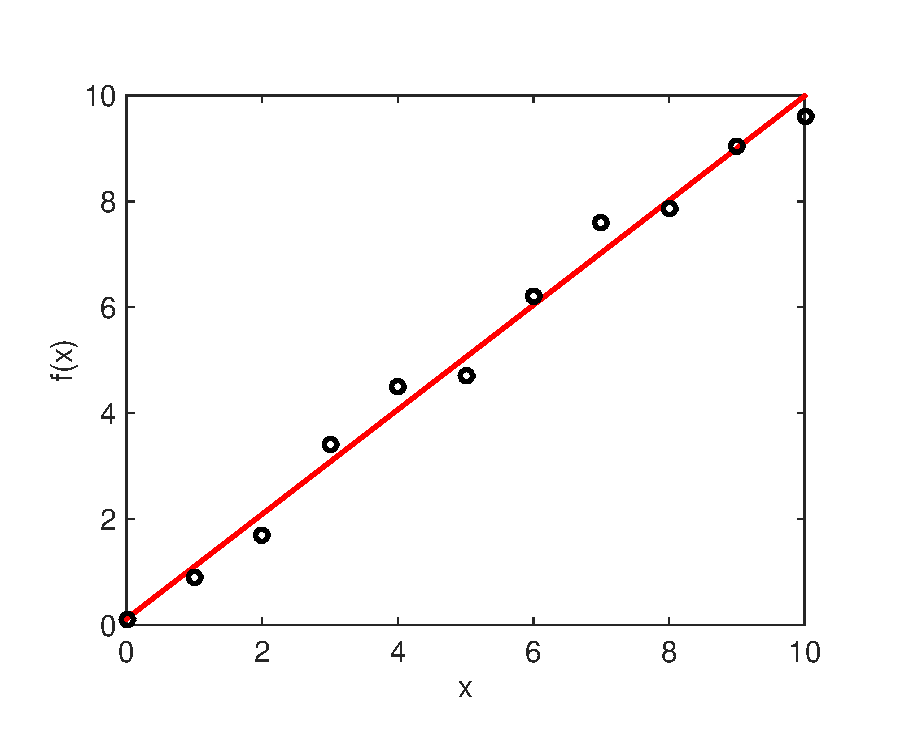
\includegraphics[width=2.5in]{12.fitting/linear_regression.pdf}
\caption{Linear regression: The solid line is obtained by the linear regression formula  (\ref{eq:linear_regression}) with $\sigma_i=1$. Despite that the data is noisy, the fitted line represents the data set very well.}\label{fig:linear_regression}
\end{figure}

We fit the data given in Table \ref{tbl:linear_regression}  with a straight line using the linear regression method.  Progrm \ref{prog:linear_regression} determines the coefficients (\ref{eq:linear_regression}).  Since no error bar is given, $\sigma_i=1$ is assumed (no discrimination).  Figure \ref{fig:linear_regression} plots the resulting curve which is fitted well to the data.

\begin{table}
\centering
\caption{Data set for Example \ref{ex:linear_regression}.}\label{tbl:linear_regression}
\begin{tabular}{c|ccccccccccc}
\hline
$x$ & 0 & 1& 2& 3& 4& 5& 6& 7& 8& 9 & 10\\
$F$ &0.1&0.90&1.7&3.4&4.5&4.7&6.2&7.6&7.85&9.03&9.6\\
\hline
\end{tabular}
\end{table}
\end{example}

\noindent
\subsection{General Linear Least Square Fitting}

It is straight forward to extend the linear regression method and fit the data with a linear combination of basis functions $u_i(x)$
\begin{equation}
f(x) = \sum_{k=1}^{M} \lambda_k u_k(x).
\end{equation}
To minimize the $\chi^2$ function, we calculate
\begin{equation}
\frac{\partial \chi^2}{\partial \lambda_j} = \frac{\partial}{\partial \lambda_j}  \sum_{i=0}^{N} \frac{1}{\sigma_i^2} \left [ \sum_{k=1}^{M} \lambda_k u_k(x_i)-\bar{f}_i \right ]^2 = 2 \sum_{i=0}^{N} \frac{u_j(x_i)}{\sigma_i^2} \left [ \sum_{k=1}^{M} \lambda_k u_k(x_i)-F_i \right ]=0 
\end{equation}
and thus
\begin{equation}
\sum_{i=0}^{N}  \sum_{k=1}^{M} \frac{u_j(x_i) u_k(x_i)}{\sigma_i^2} \lambda_k = \sum_{i=0}^{N} \frac{ u_j(x_i) F_i}{\sigma_i^2}
\end{equation}
or writing it in a matrix form
\begin{equation}\label{eq:least_square_gen}
J^\textsc{t} J\boldsymbol{\lambda} = J^\textsc{t} \mathbf{b}
\end{equation}
where 
\begin{equation}
J = \begin{bmatrix} & & \\ & J_{ij}=\displaystyle\frac{u_j(x_i)}{\sigma_i} & \\
& & \end{bmatrix}, \quad 
\boldsymbol{\lambda} = \begin{bmatrix} \lambda_1\\ \vdots \\ \lambda_{M} \end{bmatrix},\qquad
\mathbf{b} = \begin{bmatrix} F_0/\sigma_0\\ \vdots \\ F_{N}/\sigma_{N} \end{bmatrix}
\end{equation}
Note that the matrix $J$ is $N$ by $M$ and not necessarily a square matrix.  In most cases, $N \gg M$.
Noting that $J^\textsc{t} J$ is a square matrix, Eq. (\ref{eq:least_square_gen}) can be solved by Gaussian elimination or other methods in Chapter XX.

If $u_i(x) = x^i$, then $J$ is the Vandermonde matrix.  When $N=M$, it is exactly the same as the polynomial interpolation and $\chi^2=0$.  


\bigskip
\begin{example}\label{ex:quadratic_regression}

Using the least square fitting method, we fit the data given in Table \ref{tbl:quadratic_regression} with a quadratic curve.
Using the basis functions $u_1(x)=1$, $u_2(x)=x$, and $u_3(x)=x^2$, the target function is quadratic.   Program \ref{prog:quadratic_regression} implements the above method and the result is plotted in Fig. \ref{fig:quadratic_regression}.  At the data points where the error bar is small, the fitted curve is almost right on the data points.  The data points with large error bar are off the curve but most of them are within the errorbars. 

\begin{table}
\centering
\caption{Data set for Example \ref{ex:linear_regression}.}\label{tbl:quadratic_regression}
\begin{tabular}{c|ccccccccccc}
\hline
$x$ &-4.85&-3.99&-3.10&-2.10&-0.83&-0.004&0.94&1.95&2.84&4.18&4.89\\
$\bar{f}$&-47.9&-35.0&-20.5&-12.5&-1.46&1.71&-0.14&-8.09&-12.9&-37.7&-46.5\\
$\sigma$&2.2&1.8&1.2&1.8&2.9&1.7&1.2&1.5&1.3&2.2&1.7\\
\hline
\end{tabular}

\end{table}

\begin{figure}
\centering
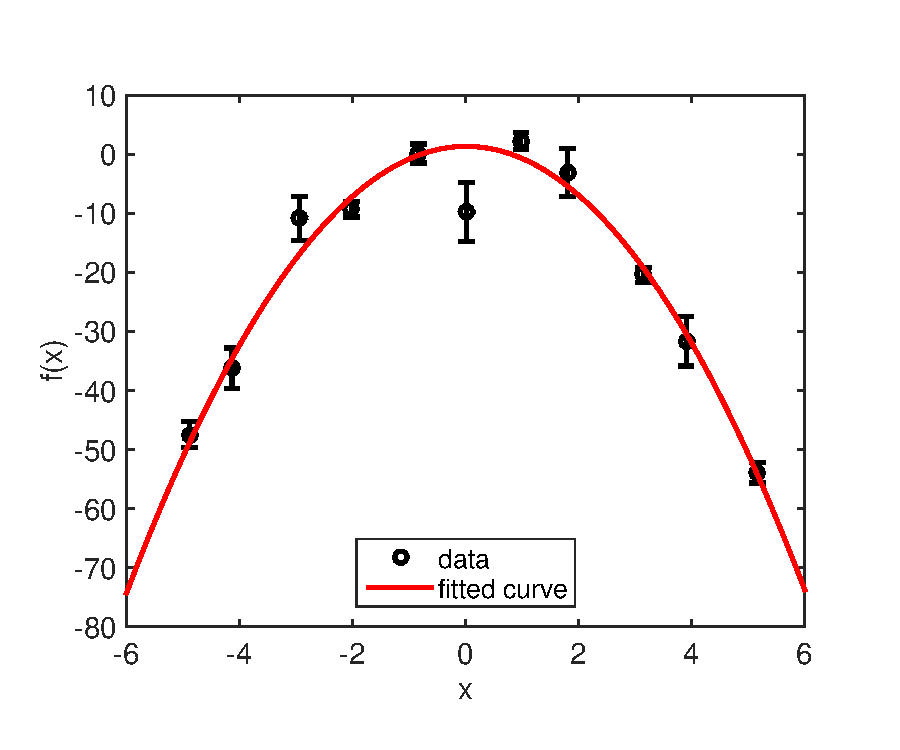
\includegraphics[width=2.5in]{12.fitting/quadratic_regression.pdf}
\caption{Least square fitting of the data set in Table \ref{tbl:quadratic_regression} with a quadratic function.  THe error bar is large where the data is close to zero.  The $\chi^2$ function allows those points to stay off the curve but not too far.}\label{fig:quadratic_regression}
\end{figure}
\end{example}


\noindent
\subsection{Nonlinear Least Square Fitting: Gauss-Newton method}

So far, the target functions are linear with the fitting parameters.  The least square fitting can be used even for nonlinear functions.
An iterative method is commonly used.  Starting with an initial guess $\lambda^{(0)}$,
we repeat the following procedure until the $\chi^2$ does not change significantly,
First, we expand the target function with respect to $\lambda$ around the current value of $\bsymb{\lambda}^{(n)}$ and keep only the first order terms:
\begin{equation}
f(x_i; \boldsymbol{\lambda}) = f(x_i; \bsymb{\lambda}^{(n)}) + \sum_{j=1}^{M} \left . \frac{\partial f(x_i;\bsymb{\lambda})}{\partial \lambda_j} \right |_{\bsymb{\lambda}^{(n)}} (\lambda_j - \lambda_j^{(n)}) = f(x_i; \bsymb{\lambda}^{(n)}) + \sum_{i=1}^{M} J_{ij}^{(n)} (\lambda_j - \lambda_j^{(n)})
\end{equation}
where the Jacobian matrix is defined by
\begin{equation}
J_{ij}^{(n)} = \left . \frac{\partial f(x_i;\bsymb{\lambda})}{\partial \lambda_j} \right |_{\bsymb{\lambda}^{(n)}}
\end{equation}
Now the target function is approximated by a linear function with respect to $\bsymb{\lambda}$.  Therefore, we can use the method discussed in Sec XX.  The residual vector is given by 
 \begin{equation}
 \Delta_i  = f(x_i; \boldsymbol{\lambda}) -F_i = f(x_i;\bsymb{\lambda}^{(n)}) + \sum_{j=1}^{M} J_{ij}^{(n)} (\lambda_j - \lambda_j^{(n)}) - F_i
 \end{equation}
 and the corresponding $\chi^2$ function is
 \begin{equation}
 \chi^2(\bsymb{\lambda}) = \sum_{i=0}^N \left (\frac{\Delta_i}{\sigma_i} \right )^2
 = \sum_{i=1}^N \frac{1}{\sigma_i}\left [f(x_i;\bsymb{\lambda}^{(n)}) + \sum_{j=1}^{M} J_{ij}^{(n)} (\lambda_j - \lambda_j^{(n)}) - \bar{f}_i \right ]^2
 \end{equation}
We minimize this $chi^2$ with respect to $\bsymb{\lambda}$ by setting the gradient to zero:
 \begin{eqnarray}
\frac{\partial \chi^2}{\partial \lambda_k} &=& 2
 \sum_{i=0}^N  J_{ik}^{(n)} \left [f(x_i;\bsymb{\lambda}^{(n)}) + \sum_{j=1}^{M} J_{ij}^{(n)} (\lambda_j - \lambda_j^{(n)}) - F_i \right ] \nonumber\\
 &=& 2 \left [ \sum_{i=0}^N \sum_{j=1}^M  J_{ik}^{(n)}  J_{ij}^{(n)} (\lambda_j - \lambda_j^{(n)}) - 
  \sum_{i=0}^N  J_{ik}^{(n)} \left \{ F_i-f(x_i;\bsymb{\lambda}^{(n)}) \right \} \right ]
 =0 
 \end{eqnarray}
 

Since this equation is linear with respect to $\bsymb{\lambda}$, we can find a new $\bsymb{\lambda}^{(n+1)}$ by solving it.  Writing the equation in matrix form
\begin{equation}
\left ( J^{(n)}\right )^\textsc{t} J^{(n)} (\bsymb{\lambda}^{(n+1)} - \bsymb{\lambda}^{(n)})  =\left ( J^{(n)}\right )^\textsc{t} \mathbf{b}
\end{equation}
the solution is
\begin{equation}\label{eq:iterative_nl_fit}
\bsymb{\lambda}^{(n+1)} = \bsymb{\lambda}^{(n)} + \left [ \left ( J^{(n)}\right )^\textsc{t} J^{(n)} \right ]^{-1} \left ( J^{(n)}\right )^\textsc{t} \mathbf{b}
\end{equation} 
where $\mathbf{b}$ is a vector whose element is $b_i=f(x_i;\bsymb{\lambda}^{(n)})-\bar{f}_i$.
Repeat the above process until you reach the minimum of $\chi^2$.   This method is called the Gauss-Newton algorithm.

 The condition to stop the iteration can be $\|\bsymb{\lambda}^{(n+1)} -
\bsymb{\lambda}^{(n)} \| < \text{tolerance}$.  However, there is a big problem.  Recall that $J^{(n)}$ becomes singular as $\chi^2$ is minimized. As the iteration proceeds, at certain point, $J^{(n)}$ becomes nearly singular and Gaussian elimination fails to find a correct solution.  Then, $\|\bsymb{\lambda}^{(n+1)} -
\bsymb{\lambda}^{(n)} \|$ starts erroneously increases.  We must stop the iteration before it happens. Usually, the solution is good enough just before the Gaussian elimination fail. In Section \ref{sec:Lorentzian}, we measure $\chi^2$ and if it goes up the iteration is terminated.   
 
The nonlinear least square fitting encounters many other difficulties.
First of all,  Eq. (\ref{eq:grad_chi2}) can have many solutions, corresponding to local minimums of the $\chi^2$ function.  The above method is not guaranteed to find the global minimum (best fit).  Some solutions are not the best fit but still reasonable.  Others are not close to the the data set at all.
Unfortunately, there is no numerical method that guarantees the global minimum.  In Chapter 18 we will discuss stochastic method that have a higher chance to find the global minimum.
Secondly, the above method often diverges because the step size is too large.  Instead of Eq. (\ref{eq:iterative_nl_fit}), update $\bsymb{\lambda}$ 
by the following equation
\begin{equation}
\bsymb{\lambda}^{(n+1)} = \bsymb{\lambda}^{(n)} + \alpha \left [ \left ( J^{(n)}\right )^\textsc{t} J^{(n)} \right ]^{-1} \left ( J^{(n)}\right )^\textsc{t} \mathbf{b}
\end{equation}
with a sufficiently small value of  $\alpha >0$.
In Section \ref{sec:Lorentzian}, we fit a Lorentzian distribution to a noisy data using the nonlinear least square fitting..



\noindent
\section{Applications in Physics}

\subsection{Arrhenius Plot}\label{sec:Arrhenius}

\begin{table}
\centering
\caption{Reaction rate $k$ as a function of absolute temperature $T$. The reaction rate is in an arbitrary unit. The bottom two rows show $\log k$ as a function pf $\beta = 1/k_\textsc{b} T$.}
\label{tbl:Arrhenius}
\begin{tabular}{c c c c c c c c c c c c}
\hline
$T$ & 200 &  220 &  240 &  260  & 280 &  300 & 320  & 340  & 360  & 380 &  400 \\
$k$ & 0.471 &    0.515&     0.576&     0.639 &    0.734 &   0.742 &   0.833 &  0.830& 0.932 &0.918&  0.939\\
\hline
$\beta$ & 58.0 &   52.7&    48.4 &   44.6 &   41.4 &   38.7 &   36.3 &   34.1 & 32.2&  30.5&   29.0\\
$\log k$ & -0.327 &  -0.288  & -0.240  & -0.194 &  -0.134 &  -0.130 &  -0.0793  & -0.0808 &-0.0307 &  -0.0371 &  -0.0273 \\
\hline
\end{tabular}

\end{table}
The temperature dependency of a chemical reaction rate is known to obey the Arrhenius equation
\begin{equation}\label{eq:Arrhenius}
k = A \me^{-E_a/k_\textsc{B} T}
\end{equation}
where $T$ and $E_a$ are the absolute temperature and an activation energy, respectively.  The temperature multiplied by the Boltzmann constant $k_\textsc{B}=8.6173324 \times 10^{-5} eV/K$ has the dimension of energy.  The constant $A$ depends on reactants but does not depend on the temperature.
Table \ref{tbl:Arrhenius} shows an experimental measurement of the reaction rate.  The data is a bit noisy.  We want to determine the activation energy of this reaction.  If we fit the data directly to the Arrhenius equation (\ref{eq:Arrhenius}), we must use a non-linear fitting, which is not a simple task. Instead, we take the logarithmic of the Arrhenius equation:
\begin{equation}\label{eq:Arrhenius_log}
\log k = - E_a \beta + log A
\end{equation}
where $\beta = 1/k_\textsc{b} T$. Equation (\ref{eq:Arrhenius_log}) indicates that $\log k$ is linear with respect to $\beta$.  Therefore, a simple linear least square fitting can determine $E_a$.
Program XXX does it.  Figure \ref{fig:Arrhenius}(a) shows that the measured data $\log k$ as a function of $\beta$ is almost straight line but significant noises are seen at higher temperature (smaller $\beta$).  The solid line determined by the least square fitting matches well to the data. Figure \ref{fig:Arrhenius}(b) plots it in the original variables $k$ vs $T$. The fitted curve represents the data very well despite it is not a strait line.  The fitting finds that the activation energy is $0.0256 eV$.

\begin{figure}
\centering
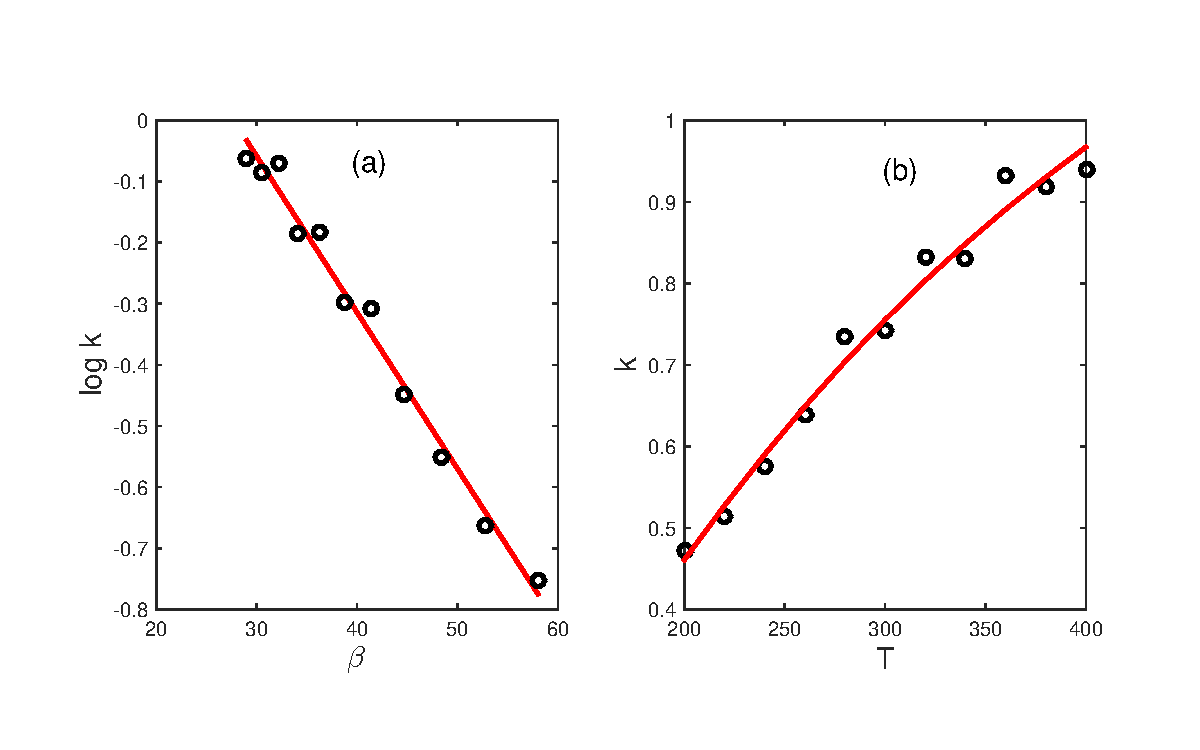
\includegraphics[width=4in]{12.fitting/arrhenius.pdf}
\caption{The least square fitting of the reaction rate.  (a) The fitting is done with variables $\log k$ and  $\beta$ sicne the theory perdict a straight line with those variables. The fitted line (solid line) matches well to the data set (open circle).  (b) The fitted curve is shown in the original variable $k$ and $T$.  The cureve is no longer a straight line but represent the data set quite well.} \label{fig:Arrhenius}
\end{figure}

\subsection{Life Time Broadening in Optical Spectrum}\label{sec:Lorentzian}

Atoms emit distinctive spectrum of light.  In the absence of thermal noise, the intensity of the light
has a peek at the frequency $\omega_0 = \Delta E /\hbar$ where $\Delta E$ is the change of electron energy in the atom.
However, the light with slightly different frequency is also observed. The excited atom has a finite life time due to the spontaneous emission of the light.  Theory predicts that the spectrum is Lorentzian
\begin{equation}
I(\omega) \propto \frac{1}{\pi} \frac{\displaystyle\frac{\Gamma}{2}}{(\omega-\omega_0)^2 + \left ( \displaystyle\frac{\Gamma}{2} \right )^2}
\end{equation}
Determining the peak position $\omega_0$ and the life time $\tau = \Gamma^{-1}$ out of the noisy experimental data is important task for experimentalists.

The data set given in Table \ref{tbl:Lorentzian} is expected to have a Lorentzian distribution:  
\begin{equation}
f(x) = \frac{\lambda_1}{(x-\lambda_2)^2+\lambda_3}.
\end{equation}
We want find the precise peak position $\lambda_2$ and the broadening $\lambda_3$ using the Gauss-Newtom method.
The derivatives of the function are given by
\begin{subequations}
\begin{eqnarray}
\frac{\partial f(x;(\boldsymbol{\lambda}))}{\partial \lambda_1} &=&  \frac{1}{(x-\lambda_2)^2+\lambda_3}\\
\frac{\partial f(x;(\boldsymbol{\lambda}))}{\partial \lambda_2} &=&  \frac{2 (x-\lambda_2)}{[(x-\lambda_2)^2+\lambda_3]^2}\\
\frac{\partial f(x;(\boldsymbol{\lambda}))}{\partial \lambda_3} &=&  \frac{-\lambda_1}{[(x-\lambda_2)^2+\lambda_3]^2}
\end{eqnarray}
\end{subequations}

The iteration begin with an initial guess $\lambda_1=1$, $\lambda_2=0$ and $\lambda_3=1$.  The $\chi^2$ function is optimized by a step factor $\alpha=0.02$.  After 40 iterations, the value of $\chi^2$ rose up and thus the iteration was terminated.  The result is plotted in Fig. (\ref{fig:Lorentzian}).  The left panel shows the raw data and the fitted curve.  The fitting appeared to be reasonable.  The right panel shows the decreasing $\chi^2$.  The converged parameter values are $\lambda_1=4.2527$, $\lambda_2=0.9442$, and $\lambda_3=3.1223$.

The Gauss-Newton method works very well for this problem.  However, the same method often completely fails for Gaussian distribution. We need more advanced method for that, which  will be introduced in Chapter 18.

\begin{table}
\centering
\caption{Data set for Lorentzian}\label{tbl:Lorentzian}
\begin{tabular}{c|ccccccccccccc}
\hline
$x$ &-2.01 & -1.47 &-0.97 &-0.52 &-0.04 &0.52 &0.99 & 1.53 & 2.03 &2.51 &2.96 &3.47 &4.02 \\
$\bar{f}$&0.28 & 0.57 &0.62 &0.68 &1.26 &1.29 &1.57 &1.11 & 0.91 &0.94 &0.65 &0.80 &0.31 \\
$\sigma$&0.10 & 0.11 &0.17 &0.06 &0.15 &0.11 &0.15 & 0.10 & 0.11 &0.14 &0.16 &0.18 &0.15 \\
\hline
\end{tabular}

\end{table}

\begin{figure}
\centering
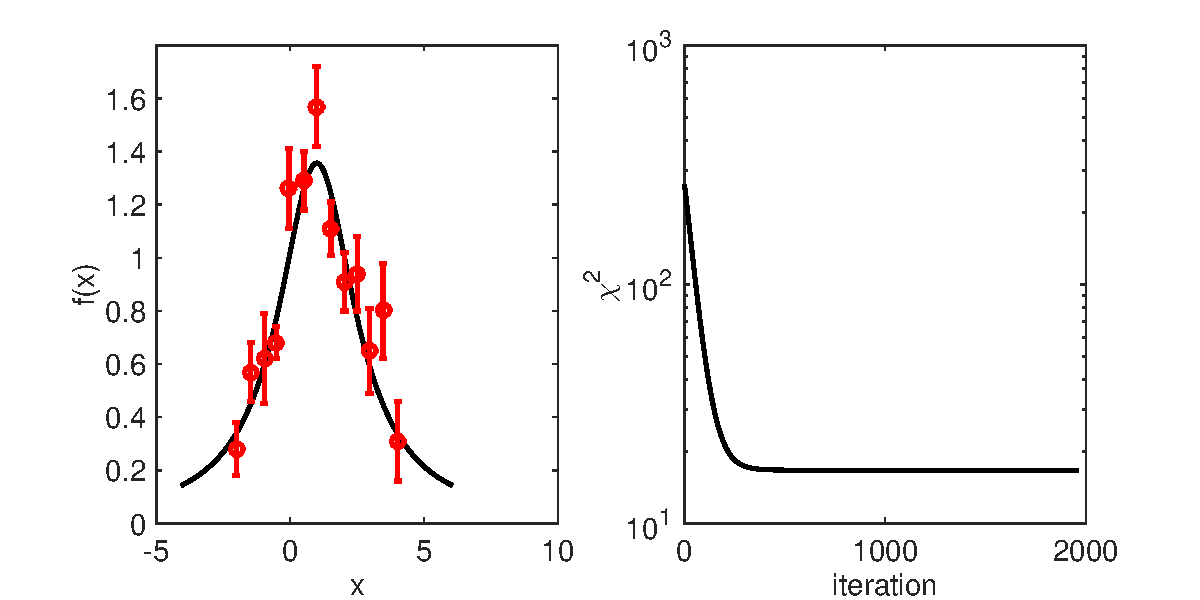
\includegraphics[width=4in]{12.fitting/lorentzian.pdf}
\caption{Nonlinear least square fitting of the noisy data set in Table \ref{tbl:Lorentzian} with a Lorentzian function.  \textit{Left}; Depite of the error bars, the Gauss-Newton method managed to fit the data to the desired function. \textit{Right}:  The $\chi^2$ decreases  as the iteration proceeds.}\label{fig:Lorentzian}
\end{figure}

\newpage
\section{Problems}


\begin{enumerate}[labelwidth=0.5cm,labelindent=0cm,leftmargin=*,label=\bfseries \thechapter.\arabic*,align=left]

\item \textbf{Life Time of Radio Active Nucleus}

A radioactive nuclide spontaneously decays to a different nuclide by emitting a particle such as $\alpha$ particle.  Suppose that there are initially $N_0$ radioactive nuclides of the same kind.  As time $t$ proceeds, the number of the nuclides decreases as
\begin{equation}
N(t) = N_0 \me^{-\lambda t}
\end{equation}
where $\lambda$ is a decay constant.  It is difficult to measure $N(t)$ directly.  However, we can detect particles emitted by the nuclides.  In experiments, we measure the number of emitted particles per second which corresponds to the decay rate\cite{decay_rate}
\begin{equation}
R(t) = - \frac{\md N}{\md t} = \lambda N_0 \me^{-\lambda t}\, .
\end{equation}

Table \ref{tbl:decay_rate} show the experimental data.  Find the decay constant using an appropriate data fitting.

\begin{table}[h]
\centering
\caption{Decay rate of a radioactive nuclide.}\label{tbl:decay_rate}
\begin{tabular}{c| c c c c c c c c c c}
\hline
t(min.) & 30&    60&    90&   120 &  150 &  180&   210&   240&   270&   300 \\
R (counts/s) & 461.9&  211.6&  103.3&   45.7&   21.7&   12.1  &  5.72 &   2.52 & 1.07 &   0.523\\
\hline
\end{tabular}
\end{table}

\end{enumerate}

\newpage

\section*{Appendix}
\addcontentsline{toc}{section}{\protect\numberline{}Appendix}

\appendix{Cubic Spline}\label{ap:cubic-spline}


\begin{equation}
q''_{i}(t) = t q''_{i} + (1-t) q^{''}_{i+1}
\end{equation}
where 
\begin{equation}
t=\displaystyle\frac{x-x_{i}}{x_{i+1}-x_{i}}
\end{equation}
\begin{equation}
q^{'}_{i}(t) = \frac{h_i}{2} t^2 q''_{i} + \frac{h_{i}}{2} t (2-t) q''_{i+1} + a_i 
\end{equation}

\begin{equation}
q_{i}(t) = \frac{h_i^2}{6} t^3 q''_{i} + \frac{h_{i}^{2}}{6} t^2 (3-t) q''_{i+1} + h_i a_i t + b_i
\end{equation}

The first condition requires that the function $q(t)$ must matches the data set.  That is $q_i(0)=\tilde{f}_i$ and $q_i(1)=\tilde{f}_{i+1}$ which leads to $a_i$ and $b_i$
\begin{subequations}
\begin{eqnarray}
a_i &=& \frac{\tilde{f}_{i+1} - \tilde{f}_i}{h_i} - \frac{h_i}{6} (2 q''_i + q''_{i+1}) \\
b_i &=& \tilde{f}_i 
\end{eqnarray}
\end{subequations}

The second condition requires that the first order derivative is continuous at the data points.  That is $q'_i(1)=q'_{i+1}(0)$, which leads to
\begin{equation}
h_i q''_{i+1} +2(h_i+h_{i-1}) q''_i + h_{i-1} q''_{i-1}  = 6 \left ( \frac{\tilde{f}_{i+1}-\tilde{f}_i}{h_i}-
\frac{\tilde{f}_i-\tilde{f}_{i-1}}{h_{i-1}} \right )
\end{equation}
At the boundary we assume $q''_1=q''_N=0$.  This is a linear equation with tridiagonal matrix.  We can solve it a method discussed in Section 7.3.1.  Now, we have all $q''_i$, $a_i$, and $b_i$.  Plugin these, we obtain $q_i(t)$ which connects data points smoothly.


\newpage
\noindent
\section*{MATLAB Source Codes}
\addcontentsline{toc}{section}{\protect\numberline{}MATLAB Source Codes}

\bigskip
\noindent

\footnotesize
\begin{verbatim}
%**************************************************************************
%*     Example 12.1                                                       *
%*     filename: ch12pr01.m                                               *
%*     program listing number: 12.1                                       *
%*                                                                        *
%*     This program interpolates 11-point data with linear spline.        *
%*                                                                        *
%*     Programed by Ryoichi Kawai for Computational Physics Course.       *
%*     Last modification:  02/25/2017.                                    *
%**************************************************************************
clear all

% data to be fitted
F=[0.0000, 0.6889, 0.6095, 0.0774, -0.3401, -0.3528,...
   -0.0842, 0.1620, 0.1997, 0.0681, -0.0736];
X=[0.0,1.0,2.0,3.0,4.0,5.0,6.0,7.0,8.0,9.0,10.];
N=size(F,2)-1;
h=X(2:N+1)-X(1:N);

M=10;
dt=1.0/M;
t=linspace(0.,dt*(M-1),M);

n=0;
for i=1:N-1
    % linear interpolation between two adjacent data points
    for j=1:M
        n=n+1;
        x(n)=t(j)*h(i)+X(i);
        y(n)=(1-t(j))*F(i)+t(j)*F(i+1);
    end
end

n=n+1;
x(n)=X(N+1);
y(n)=F(N+1);
z=sin(x).*exp(-0.2*x);

p=plot(x,y,X,F,'o',x,z,'--');
set(p,'linewidth',2);
xlabel('x','fontsize',14);
ylabel('f(x)','fontsize',14);
legend('Spline','Data','Original');
legend('location','northeast');
\end{verbatim}
\normalsize

\ruleend
\bigskip
\noindent
\program
\label{prog:spline_cubic}
\footnotesize
\begin{verbatim}
%**************************************************************************
%*     Example 12.2                                                       *
%*     filename: ch12pr02.m                                               *
%*     program listing number: 12.2                                       *
%*                                                                        *
%*     This program interpolates 11-point data with cubic spline.         *
%*                                                                        *
%*     Programed by Ryoichi Kawai for Computational Physics Course.       *
%*     Last modification:  02/25/2017.                                    *
%**************************************************************************
clear all

% data to be fitted
F=[0.0000, 0.6889, 0.6095, 0.0774, -0.3401, -0.3528,...
   -0.0842, 0.1620, 0.1997, 0.0681, -0.0736];
X=[0.0,1.0,2.0,3.0,4.0,5.0,6.0,7.0,8.0,9.0,10.];
N=size(F,2)-1;
h=X(2:N+1)-X(1:N);

% Set up linear equation A*P=G
for j=1:N-1
    G(j)=3*((F(j+2)-F(j+1))/h(j+1)-(F(j+1)-F(j))/h(j));
end

A=zeros(N-2,N-2);
for j=1:N-1
    A(j,j)=(h(j+1)+h(j))/2;
end
for j=1:N-2
    A(j,j+1)=h(j+1);
    A(j+1,j)=h(j+1);
end

P=A\G'; %Solve the linear equation

% Shift the index to our convention.
for j=1:N-1
    Q(j+1)=P(j);
end

% Amend the boundary values.
Q(1)=0;
Q(N+1)=0;

M=10;
dt=1.0/M;
t=linspace(0.,dt*(M-1),M);

n=0;
for k=1:N
    for j=1:M
        n=n+1;
        x(n)=X(k)+t(j)*h(k);
        y(n)=h(k)^2/6 * Q(k)   * t(j)*(t(j)+1)*(t(j)-1) ...
            -h(k)^2/6 * Q(k+1) * t(j)*(t(j)-1)*(t(j)-2) ...
            +F(k+1)*t(j) + (1-t(j))*F(k);
    end
end

v=sin(x).*exp(-0.2*x);
p=plot(x,y,X,F,'o',x,v,'--');
set(p,'linewidth',2);
xlabel('x','fontsize',14);
ylabel('f(x)','fontsize',14);
legend('Cubic Spline','Data ', 'Original');
legend('location','northeast');
\end{verbatim}
\normalsize

\ruleend
\bigskip
\noindent
\program
\label{prog:vandermonde}
\footnotesize
\begin{verbatim}
%**************************************************************************
%*     Example 12.3                                                       *
%*     filename: ch12pr03.m                                               *
%*     program listing number: 12.3                                       *
%*                                                                        *
%*     This program interpolates 11-point data with the Vandermonde       *
%*     matrix.                                                            *
%*                                                                        *
%*     Programed by Ryoichi Kawai for Computational Physics Course.       *
%*     Last modification:  02/25/2017.                                    *
%**************************************************************************
clear all

% data to be fitted
F=[0.0000, 0.6889, 0.6095, 0.0774, -0.3401, -0.3528,...
   -0.0842, 0.1620, 0.1997, 0.0681, -0.0736];
X=[0.0,1.0,2.0,3.0,4.0,5.0,6.0,7.0,8.0,9.0,10.];
N=size(F,2);

% construction of the Vandermonde matrix
x = zeros(N,N);
x(:,1)=1;
for i=2:N
    x(:,i)=X(:).^(i-1);
end

% solve the linear equation x*a=F
a=x\F';

% evaluate the function value
% between the sampling points.
M=101;
z=linspace(0,X(N),M);

for j=1:M
    y(j)=a(1);
    for i=2:N
        y(j)=y(j)+a(i)*z(j)^(i-1);
    end
end

v = sin(z).*exp(-0.2*z);

p=plot(X,F,'o',z,y,z,v,'--');
set(p,'linewidth',2);
xlabel('x','fontsize',14);
ylabel('f(x)','fontsize',14);
legend('Data','Vandermonde fit','Original');
legend('location','northeast');
\end{verbatim}
\normalsize

\ruleend
\bigskip
\noindent
\program
\label{prog:lagrange_poly}
\footnotesize
\begin{verbatim}
%**************************************************************************
%*     Example 12.4                                                       *
%*     filename: ch12pr04.m                                               *
%*     program listing number: 12.4                                       *
%*                                                                        *
%*     This program interpolates 11-point data with the Lagrange          *
%*     polynomial method.                                                 *
%*                                                                        *
%*     Programed by Ryoichi Kawai for Computational Physics Course.       *
%*     Last modification:  02/25/2017.                                    *
%**************************************************************************
clear all

% data to be fitted
F=[0.0000, 0.6889, 0.6095, 0.0774, -0.3401, -0.3528,...
   -0.0842, 0.1620, 0.1997, 0.0681, -0.0736];
X=[0.0,1.0,2.0,3.0,4.0,5.0,6.0,7.0,8.0,9.0,10.];
N=size(F,2);

M=101;
z=linspace(0,X(N),M);
for j=1:M
    L=1;
    y(j)=0;
    for n=1:N
        L=1; % Lagrange basis polynomial
        for m=1:N
            if n~=m
                L=L*(z(j)-X(m))/(X(n)-X(m));
            end
        end
        y(j)=y(j)+L*F(n);
    end
end

v=sin(z).*exp(-0.2*z);

p=plot(X,F,'o',z,y,z,v,'--');
set(p,'linewidth',2);
xlabel('x','fontsize',14);
ylabel('f(x)','fontsize',14);
legend('Data','Lagrange polynomial','Original');
legend('location','northeast');
\end{verbatim}
\normalsize

\ruleend
\bigskip
\noindent
\program
\label{prog:linear_regression}
\footnotesize
\begin{verbatim}
%**************************************************************************
%*     Example 12.5                                                       *
%*     filename: ch12pr05.m                                               *
%*     program listing number: 12.5                                       *
%*                                                                        *
%*     This program interpolates 11-point data with the linear            *
%*     regression method.                                                 *
%*                                                                        *
%*     Programed by Ryoichi Kawai for Computational Physics Course.       *
%*     Last modification:  02/25/2017.                                    *
%**************************************************************************
clear all;

% Data set (no error bar)
x=[0.0,1.0,2.0,3.0,4.0,5.0,6.0,7.0,8.0,9.0,10.];
y=[0.1,0.90,1.7,3.4,4.5,4.7,6.2,7.6,7.85,9.03,9.6];
N=size(y,2);

% Linear regression
F=sum(y);
X=sum(x);
X2=sum(x.^2);
XF=sum(x.*y);
b=(F*X2-X*XF)/(N*X2-X^2);
a=(N*XF-X*F)/(N*X2-X^2);

% fitted curve
f=a*x+b;

p=plot(x,f);
set(p,'linewidth',2,'color','red')
hold on
r=plot(x,y,'o');
set(r,'linewidth',2,'color','black')
xlabel('x','fontsize',14)
ylabel('f(x)','fontsize',14)
hold off
\end{verbatim}
\normalsize

\ruleend
\bigskip
\noindent
\program
\label{prog:quadratic_regression}
\footnotesize
\begin{verbatim}
%**************************************************************************
%*     Example 12.6                                                       *
%*     filename: ch12pr06.m                                               *
%*     program listing number: 12.6                                       *
%*                                                                        *
%*     This program interpolates 11-point data with the quadratic         *
%*     regression method.                                                 *
%*                                                                        *
%*     Programed by Ryoichi Kawai for Computational Physics Course.       *
%*     Last modification:  02/25/2017.                                    *
%**************************************************************************
clear all

% Generate a noisy data set
N=13;
sm=5.0;
for i=1:N
    x(i)=i-7.+random('unif',-0.2,0.2);
    s(i)=random('norm',0,sm/2)+sm;
    y(i)=-2*x(i)^2+s(i)*random('unif',0.2,0.9);
end

M=3; % number of parameters

% Construct Jacobian matrix and a vector
for i=1:N
    for j=1:M
        J(i,j)=x(i)^(j-1)/s(i);
    end
    b(i)=y(i)/s(i);
end

% Solve the linear equation
A=J'*J;
c=J'*b';
lambda=A\c;

% constructe the fitted curve
K=121;
z=linspace(-6.0,6.0,K);
f=lambda(1)+lambda(2)*z+lambda(3)*z.^2;

r=errorbar(x,y,s,'o');
set(r,'linewidth',2,'color','black')
hold on

p=plot(z,f);
set(p,'linewidth',2,'color','red')
xlabel('x','fontsize',14)
ylabel('f(x)','fontsize',14)
legend('data','fitted curve')
legend('location','south')
xlim([-7 7]);
hold off
\end{verbatim}
\normalsize

\ruleend
\bigskip
\noindent
\program
\label{prog:Arrhenius}
\footnotesize
\begin{verbatim}
%**************************************************************************
%*     Section 12.3.1                                                     *
%*     filename: ch12pr07.m                                               *
%*     program listing number: 12.7                                       *
%*                                                                        *
%*     This program finds the activation energy of a reaction from a data *
%*     set using the linear regression.                                   *
%*                                                                        *
%*     Programed by Ryoichi Kawai for Computational Physics Course.       *
%*     Last modification:  02/25/2017.                                    *
%**************************************************************************
clear all;

k=8.617e-5; % Boltzmann constant [eV/K]

% Generate a new dataset
%E=0.025;
%A=2.0;
%for i=1:11
%    T(i) = 180+20*i;
%    f(i)=2.0*exp(-E/(k*T(i)))*(1+random('unif',-0.05,+0.05));
%end

T=[200, 220, 240, 260, 280, 300, 320, 340, 360, 380, 400];
f=[0.471,0.515,0.576,0.639,0.734,0.742,0.833,0.830,0.932,0.918,0.939];
N=size(f,2);

for i=1:N
    x(i)=1/(k*T(N+1-i));
    y(i)=log(f(N+1-i));
end

F=sum(y);
X=sum(x);
X2=sum(x.^2);
XF=sum(x.*y);
b=(F*X2-X*XF)/(N*X2-X^2);
a=(N*XF-X*F)/(N*X2-X^2);
g=a*x+b;
A=exp(b);
z = A*exp(a./(k*T));

fprintf('Activation Energy = %6.2d eV\n',abs(a))

subplot(1,2,1)
p=plot(x,g);
set(p,'linewidth',2,'color','red')
hold on
r=plot(x,y,'o');
set(r,'linewidth',2,'color','black')
xlabel(texlabel('beta'),'fontsize',14)
ylabel('log k','fontsize',14)
hold off
subplot(1,2,2)
p=plot(T,f,'o');
set(p,'linewidth',2,'color','black')
hold on
r=plot(T,z);
set(r,'linewidth',2,'color','red')
xlabel('T','fontsize',14)
ylabel('k','fontsize',14)
hold off
\end{verbatim}
\normalsize

\ruleend
\bigskip
\noindent
\program
\label{prog:Lorentzian}
\footnotesize
\begin{verbatim}
%**************************************************************************
%*     Section 12.3.2                                                     *
%*     filename: ch12pr08.m                                               *
%*     program listing number: 12.8                                       *
%*                                                                        *
%*     This program finds the peak position and life-time broadening      *
%*     of atomic emmision spectrum.                                       *
%*                                                                        *
%*     Programed by Ryoichi Kawai for Computational Physics Course.       *
%*     Last modification:  02/25/2017.                                    *
%**************************************************************************
clear all;

% Generate a sample noisy data

x=[-2.01,-1.47,-0.97,-0.52,-0.04,0.52,0.99,1.53,2.03,2.51,2.96,3.47,4.02];
y=[0.28,0.57,0.62,0.68,1.26,1.29,1.57,1.11,0.91,0.94,0.65,0.80,0.31];
s=[0.10,0.11,0.17,0.06,0.15,0.11,0.15,0.10,0.11,0.14,0.16,0.18,0.15];
N=size(y,2);

%control parametrs
alpha=1e-2;
found=false;

%initial guess
M=3;
lambda(:,1)=[1,0,1];

% Gauss-Newton iteration
n=1;
% evaluate initial chi sqaure
for i=1:N
   F=lambda(1,n)/((x(i)-lambda(2,n))^2+lambda(3,n));
   b(i)=y(i)-F;
end
b=b./s;
chi2(n)=b*b';

while not(found)
    % construct Jacobian and vectors.
    for i=1:N
        F=lambda(1,n)/((x(i)-lambda(2,n))^2+lambda(3,n));
        J(i,1)=F/lambda(1,n);
        J(i,2)=2*lambda(1,n)*(x(i)-lambda(2,n))...
              /((x(i)-lambda(2,n))^2+lambda(3,n))^2;
        J(i,3)=-lambda(1,n)/((x(i)-lambda(2,n))^2+lambda(3,n))^2;
        b(i)=y(i)-F;
    end
    % Take into account error bar
    b=b./s;
    for i=1:M
       J(:,i)=J(:,i)./s';
    end
   
    % Solve the equation
    n=n+1;
    A=J'*J;
    c=J'*b';
    d=A\c;
    
    % update parameter values
    lambda(:,n)=lambda(:,n-1)+alpha*d;
    % evaluate chi sqaure
    chi2(n)=b*b';    

    % if chi square goes up stop
    if chi2(n)-chi2(n-1) > 0
        found=true;
    end
end

subplot(1,2,1)
z=[-4:0.1:6];
L=size(z,2);
for i=1:L
w(i)=lambda(1,n)/((z(i)-lambda(2,n))^2+lambda(3,n));
end
p=plot(z,w);
set(p,'linewidth',2,'color','black')
hold on
r=errorbar(x,y,s,'o');
set(r,'linewidth',2,'color','red')
xlabel('x','fontsize',14)
ylabel('f(x)','fontsize',14)
hold off

subplot(1,2,2)
r=semilogy([1:n],chi2);
set(r,'linewidth',2,'color','black')
xlabel('iteration','fontsize',14)
ylabel(texlabel('chi^2'),'fontsize',14)
\end{verbatim}
\normalsize

\ruleend

\bigskip
\noindent
\section*{Python Source Codes}
\addcontentsline{toc}{section}{\protect\numberline{}Python Source Codes}
\setcounter{program}{0}

\bigskip
\noindent
\program
\footnotesize
\begin{verbatim}
#!/usr/bin/env python3
# -*- coding: utf-8 -*-
"""
%**************************************************************************
%*     Example 12.1                                                       *
%*     filename: ch12pr01.py                                              *
%*     program listing number: 12.1                                       *
%*                                                                        *
%*     This program interpolates 11-point data with linear spline.        *
%*                                                                        *
%*     Programed by Ryoichi Kawai for Computational Physics Course.       *
%*     Last modification:  02/25/2017.                                    *
%**************************************************************************
"""
import numpy as np
import matplotlib.pyplot as plt

# data to be fitted
F=[0.0000, 0.6889, 0.6095, 0.0774, -0.3401, -0.3528,\
   -0.0842, 0.1620, 0.1997, 0.0681, -0.0736]
X=[0.0,1.0,2.0,3.0,4.0,5.0,6.0,7.0,8.0,9.0,10.]
F=np.array(F)
X=np.array(X)
N=F.size # Num er of data points
h=np.zeros(N-1)
for j in range(0,N-1):
    h[j]=X[j+1]-X[j]

M=10  # Number of interpolation points between data points
dt=1.0/M
T=np.linspace(0.0,dt*(M-1),M) # linear interpolation

x=np.zeros(N*M)
y=np.zeros(N*M)

n=0
for i in range(0,N-1):
    # linear interpolation between two adjacent data points
    for t in T:
        x[n]=t*h[i]+X[i]
        y[n]=(1.0-t)*F[i]+t*F[i+1]
        n+=1

x[n]=X[N-1]
y[n]=F[N-1]
z=np.sin(x)*np.exp(-0.2*x)

n+=1
plt.figure(figsize=(6,5))
plt.plot(x[0:n],y[0:n],'-r',label='Spline')
plt.plot(X,F,'ob',label='Data')
plt.plot(x[0:n],z[0:n],'--k',label='Source')
plt.xlabel('x',fontsize=14)
plt.ylabel('f(x)',fontsize=14)
plt.legend(loc=1)
plt.show()
\end{verbatim}
\normalsize

\ruleend


\bigskip
\noindent
\program
\footnotesize
\begin{verbatim}
#!/usr/bin/env python3
# -*- coding: utf-8 -*-
"""
%**************************************************************************
%*     Example 12.2                                                       *
%*     filename: ch12pr02.py                                              *
%*     program listing number: 12.2                                       *
%*                                                                        *
%*     This program interpolates 11-point data with cubic spline.         *
%*                                                                        *
%*     Programed by Ryoichi Kawai for Computational Physics Course.       *
%*     Last modification:  02/25/2017.                                    *
%**************************************************************************
"""
import numpy as np
import matplotlib.pyplot as plt

# data to be fitted
F=[0.0000, 0.6889, 0.6095, 0.0774, -0.3401, -0.3528,\
   -0.0842, 0.1620, 0.1997, 0.0681, -0.0736]
X=[0.0,1.0,2.0,3.0,4.0,5.0,6.0,7.0,8.0,9.0,10.]
F=np.array(F)
X=np.array(X)
N=F.size
h=np.zeros(N-1)
for j in range(0,N-1):
    h[j]=X[j+1]-X[j]

G=np.zeros(N-2)
for j in range(0,N-2):
    G[j]=3*((F[j+2]-F[j+1])/h[j+1]-(F[j+1]-F[j])/h[j])

A=np.zeros((N-2,N-2))
for j in range(0,N-2):
    A[j,j]=(h[j+1]+h[j])/2.0

for j in range(0,N-3):
    A[j,j+1]=h[j+1]
    A[j+1,j]=h[j+1]

P=np.linalg.solve(A,G)

Q=np.zeros(N)
for j in range(0,N-2):
    Q[j+1]=P[j]

Q[0]=0.0
Q[N-1]=0.0

M=10  # Number of interpolation points between data points
dt=1.0/M
T=np.linspace(0.0,dt*(M-1),M) # linear interpolation
x=np.zeros(N*M)
y=np.zeros(N*M)
n=0
for i in range(0,N-1):
    # linear interpolation between two adjacent data points
    for t in T:
        x[n]=t*h[i]+X[i]
        y[n]=h[i]**2/6.0 * Q[i]   * t*(t+1.0)*(t-1.0) \
            -h[i]**2/6.0 * Q[i+1] * t*(t-1.0)*(t-2.0) \
            +F[i+1]*t + (1.0-t)*F[i]
        n+=1

z=np.sin(x[0:n])*np.exp(-0.2*x[0:n])

plt.figure(figsize=(6,5))
plt.plot(x[0:n],y[0:n],'-r',label='Spline')
plt.plot(X,F,'ob',label='Data')
plt.plot(x[0:n],z[0:n],'--k',label='Source')
plt.xlabel('x',fontsize=14)
plt.ylabel('f(x)',fontsize=14)
plt.legend(loc=1)
plt.show()
\end{verbatim}
\normalsize

\ruleend

\bigskip
\noindent
\program
\footnotesize
\begin{verbatim}
#!/usr/bin/env python3
# -*- coding: utf-8 -*-
"""
%**************************************************************************
%*     Example 12.3                                                       *
%*     filename: ch12pr03.py                                              *
%*     program listing number: 12.3                                       *
%*                                                                        *
%*     This program interpolates 11-point data with the Vandermonde       *
%*     matrix.                                                            *
%*                                                                        *
%*     Programed by Ryoichi Kawai for Computational Physics Course.       *
%*     Last modification:  02/24/2017.                                    *
%**************************************************************************
"""
import numpy as np
import matplotlib.pyplot as plt

F=[0.0000, 0.6889, 0.6095, 0.0774, -0.3401, -0.3528,\
   -0.0842, 0.1620, 0.1997, 0.0681, -0.0736]
X=[0.0,1.0,2.0,3.0,4.0,5.0,6.0,7.0,8.0,9.0,10.]
F=np.array(F)
X=np.array(X)
N=F.size

# construction of the Vandermonde matrix
x = np.zeros((N,N))
x[:,0]=1.0
for n in range(1,N):
    x[:,n]=X[:]**n

# solve the linear equation
# using Gaussian elimination
a=np.linalg.solve(x,F)

# evaluate the function value
# between the sampling points.

M=101
z=np.linspace(0.0,X[N-1],M)
y=np.zeros(M)

for j in range(0,M):
    y[j]=a[0]
    for i in range(1,N):
        y[j]=y[j]+a[i]*z[j]**i

v = np.sin(z)*np.exp(-0.2*z)

plt.figure(figsize=(6,5))
plt.plot(X,F,'ob',label="Raw data")
plt.plot(z,y,'-r',label="Vandermonde")
plt.plot(z,v,'--k',label="Source")
plt.xlabel('x',fontsize=14)
plt.ylabel('f(x)',fontsize=14)
plt.legend(loc=1)
plt.show()
\end{verbatim}
\normalsize

\ruleend

\bigskip
\noindent
\program
\footnotesize
\begin{verbatim}
#!/usr/bin/env python3
# -*- coding: utf-8 -*-
"""
%**************************************************************************
%*     Example 12.4                                                       *
%*     filename: ch12pr04.py                                              *
%*     program listing number: 12.4                                       *
%*                                                                        *
%*     This program interpolates 11-point data with the Lagrange          *
%*     polynomial method.                                                 *
%*                                                                        *
%*     Programed by Ryoichi Kawai for Computational Physics Course.       *
%*     Last modification:  02/25/2017.                                    *
%**************************************************************************
"""
import numpy as np
import matplotlib.pyplot as plt

# data to be fitted
F=[0.0000, 0.6889, 0.6095, 0.0774, -0.3401, -0.3528,\
   -0.0842, 0.1620, 0.1997, 0.0681, -0.0736]
X=[0.0,1.0,2.0,3.0,4.0,5.0,6.0,7.0,8.0,9.0,10.]
F=np.array(F)
X=np.array(X)
N=F.size

M=101
z=np.linspace(0.0,X[N-1],M)
y=np.zeros(M)

for j in range(0,M):

    for n in range(0,N):
        L=1.0   # Lagrange basis polynomial
        for m in range(0,N):
            if n!=m:
                L=L*(z[j]-X[m])/(X[n]-X[m])

        y[j]=y[j]+L*F[n]

v=np.sin(z)*np.exp(-0.2*z)

plt.figure(figsize=(6,5))
plt.plot(X,F,'ob',label="Raw data")
plt.plot(z,y,'-r',label="Lagrange")
plt.plot(z,v,'--k',label="Source")
plt.xlabel('x',fontsize=14)
plt.ylabel('f(x)',fontsize=14)
plt.legend(loc=1)
plt.show()
\end{verbatim}
\normalsize

\ruleend

\bigskip
\noindent
\program
\footnotesize
\begin{verbatim}
#!/usr/bin/env python3
# -*- coding: utf-8 -*-
"""
%**************************************************************************
%*     Example 12.5                                                       *
%*     filename: ch12pr05.py                                              *
%*     program listing number: 12.5                                       *
%*                                                                        *
%*     This program interpolates 11-point data with the linear            *
%*     regression method.                                                 *
%*                                                                        *
%*     Programed by Ryoichi Kawai for Computational Physics Course.       *
%*     Last modification:  02/25/2017.                                    *
%**************************************************************************
"""
import numpy as np
import matplotlib.pyplot as plt

# Data set (no error bar)

x=[0.0,1.0,2.0,3.0,4.0,5.0,6.0,7.0,8.0,9.0,10.]
y=[0.1,0.90,1.7,3.4,4.5,4.7,6.2,7.6,7.85,9.03,9.6]
x=np.array(x)
y=np.array(y)
N=y.size

# Linear regression
F=y.sum()
X=x.sum()
X2=(x**2).sum()
XF=(x*y).sum()
b=(F*X2-X*XF)/(N*X2-X**2)
a=(N*XF-X*F)/(N*X2-X**2)

# fitted curve
f=a*x+b

plt.figure(figsize=(6,5))
plt.plot(x,f,'-r')
plt.plot(x,y,'ok');
plt.xlabel('x',fontsize=14)
plt.ylabel('f(x)',fontsize=14)
plt.show()
\end{verbatim}
\normalsize

\ruleend

\bigskip
\noindent
\program
\footnotesize
\begin{verbatim}
#!/usr/bin/env python3
# -*- coding: utf-8 -*-
"""
%**************************************************************************
%*     Example 12.6                                                       *
%*     filename: ch12pr06.py                                              *
%*     program listing number: 12.6                                       *
%*                                                                        *
%*     This program interpolates 11-point data with the quadratic         *
%*     regression method.                                                 *
%*                                                                        *
%*     Programed by Ryoichi Kawai for Computational Physics Course.       *
%*     Last modification:  02/25/2017.                                    *
%**************************************************************************
"""
import numpy as np
import matplotlib.pyplot as plt

# Generate a noisy data set
N=13
x=np.zeros(N)
y=np.zeros(N)
s=np.zeros(N)
sm=5.0
for i in range(0,N):
    x[i]=i-6.+np.random.uniform(-0.2,0.2)
    s[i]=np.random.normal(0.0,sm/2.)+sm
    y[i]=-2*x[i]**2+s[i]*np.random.uniform(0.2,0.9)

M=3; # number of parameters
J=np.matrix(np.zeros((N,M)))
b=np.matrix(np.zeros(N)).transpose()

# Construct Jacobian matrix and a vector
for i in range(0,N):
    for j in range(0,M):
        J[i,j]=x[i]**j/s[i]

    b[i]=y[i]/s[i]

# Solve the linear equation
A=J.transpose()*J
c=J.transpose()*b
lam=np.linalg.solve(A,c)

# constructe the fitted curve
K=121
z=np.linspace(-6.0,6.0,K)
f=lam[0,0]+lam[1,0]*z+lam[2,0]*z**2

plt.figure(figsize=(6,5))
plt.errorbar(x,y,yerr=s,fmt='ok',label='Data')
plt.plot(z,f,'-r',label='Fit')
plt.xlabel('x',fontsize=14)
plt.ylabel('f(x)',fontsize=14)
plt.legend(loc=1)
plt.show()
\end{verbatim}
\normalsize

\ruleend

\bigskip
\noindent
\program
\footnotesize
\begin{verbatim}
#!/usr/bin/env python3
# -*- coding: utf-8 -*-
"""
%**************************************************************************
%*     Section 12.3.1                                                     *
%*     filename: ch12pr07.py                                               *
%*     program listing number: 12.7                                       *
%*                                                                        *
%*     This program finds the activation energy of a reaction from a data *
%*     set using the linear regression.                                   *
%*                                                                        *
%*     Programed by Ryoichi Kawai for Computational Physics Course.       *
%*     Last modification:  02/25/2017.                                     *
%**************************************************************************
"""
import numpy as np
import matplotlib.pyplot as plt

k=8.617e-5; # Boltzmann constant [eV/K]

T=[200., 220., 240., 260., 280., 300., 320., 340., 360., 380., 400.]
f=[0.471,0.515,0.576,0.639,0.734,0.742,0.833,0.830,0.932,0.918,0.939]
f=np.array(f)
T=np.array(T)
N=f.size
x=1./(k*T[::-1])   
y=np.log(f[::-1])

# Linear regression
F=y.sum()
X=x.sum()
X2=(x**2).sum()
XF=(x*y).sum()
b=(F*X2-X*XF)/(N*X2-X**2)
a=(N*XF-X*F)/(N*X2-X**2)

g=a*x+b
A=np.exp(b)
z = A*np.exp(a/(k*T))

print('\nActivation Energy = {0:8.4f} eV\n'.format(np.abs(a)))

plt.figure(figsize=(12,5))
plt.subplot(1,2,1)
plt.plot(x,g,'-r')
plt.plot(x,y,'ok')
plt.xlabel(r'$\beta$',fontsize=14)
plt.ylabel(r'$\log\, k$',fontsize=14)

plt.subplot(1,2,2)
plt.plot(T,f,'ok')
plt.plot(T,z,'-r')
plt.xlabel('T',fontsize=14)
plt.ylabel('k',fontsize=14)
plt.show()
\end{verbatim}
\normalsize

\ruleend

\bigskip
\noindent
\program
\footnotesize
\begin{verbatim}
#!/usr/bin/env python3
# -*- coding: utf-8 -*-
"""
%**************************************************************************
%*     Section 12.3.2                                                     *
%*     filename: ch12pr08.m                                               *
%*     program listing number: 12.8                                       *
%*                                                                        *
%*     This program finds the peak position and life-time broadening      *
%*     of atomic emmision spectrum.                                       *
%*                                                                        *
%*     Programed by Ryoichi Kawai for Computational Physics Course.       *
%*     Last modification:  02/25/2017.                                    *
%**************************************************************************
"""
import numpy as np
import matplotlib.pyplot as plt

# Generate a sample noisy data
x=[-2.01,-1.47,-0.97,-0.52,-0.04,0.52,0.99,1.53,2.03,2.51,2.96,3.47,4.02]
y=[0.28,0.57,0.62,0.68,1.26,1.29,1.57,1.11,0.91,0.94,0.65,0.80,0.31]
s=[0.10,0.11,0.17,0.06,0.15,0.11,0.15,0.10,0.11,0.14,0.16,0.18,0.15]

x=np.array(x)
y=np.array(y)
s=np.array(s)
N=x.size

# control parametrs
alpha=1.e-2


# initial guess
K=2000
M=3
lam=np.zeros((K,M))
chi2=np.zeros(K)

lam[0,:]=np.array([1.,0.,1.])

# Gauss-Newton iteration
n=0
# evaluate initial chi sqaure
b=np.zeros(N)
J=np.zeros((N,M))

for i in range(0,N):
   F=lam[n,0]/((x[i]-lam[n,1])**2+lam[n,2])
   b[i]=y[i]-F

b=b/s
chi2[n]=(b**2).sum()


found=False
while not(found):
    # construct Jacobian and vectors.
    for i in range(0,N): 
        F=lam[n,0]/((x[i]-lam[n,1])**2+lam[n,2])
        J[i,0]=F/lam[n,0]
        J[i,1]=2.*lam[n,0]*(x[i]-lam[n,1])\
              /((x[i]-lam[n,1])**2+lam[n,2])**2
        J[i,2]=-lam[n,0]/((x[i]-lam[n,1])**2+lam[n,2])**2
        b[i]=y[i]-F

    # Take into account error bar
    b=b/s
    for i in range(0,M):
       J[:,i]=J[:,i]/s
   
    # Solve the equation
    n+=1
    A=np.dot(J.transpose(),J)
    c=np.dot(J.transpose(),b)
    d=np.linalg.solve(A,c)
    
    # update parameter values
    lam[n,:]=lam[n-1,:]+alpha*d
    # evaluate chi sqaure
    chi2[n]=(b**2).sum()    

    # if chi square goes up stop
    if chi2[n]-chi2[n-1] > 0:
        found=True

        
plt.figure(figsize=(12,5))
plt.subplot(1,2,1)
z=np.linspace(-4.0,6.0,101)
L=z.size
w=np.zeros(L)

for i in range(0,L):
    w[i]=lam[n,0]/((z[i]-lam[n,1])**2+lam[n,2])

plt.plot(z,w)
plt.errorbar(x,y,yerr=s,fmt='o')
plt.xlabel('x',fontsize=14)
plt.ylabel('f(x)',fontsize=14)

plt.subplot(1,2,2)
plt.semilogy(np.linspace(1,n,n),chi2[0:n])
plt.xlabel('iteration',fontsize=14)
plt.ylabel(r'$\chi^2$',fontsize=14)
plt.show()
\end{verbatim}
\normalsize

\ruleend

\vfill

\newpage
%\chapbibliography
\bibliographystyle{unsrt}
\bibliography{compphys}
